% !TEX program = pdflatex
% 夫兰克-赫兹实验 实验报告
\documentclass[UTF8,10pt,a4paper]{article}
\usepackage{ctex}
% \catcode`\。=\active
% \newcommand{。}{.}
\newcommand{\CourseName}{近代物理实验}
\newcommand{\CourseCode}{PHYS1701}
\newcommand{\Semester}{2019-2020学年第学期}
\newcommand{\ProjectName}{夫兰克-赫兹实验 报告}
\newcommand{\TimeType}{实验日期}
\newcommand{\Time}{2020. 6. 3(周三)}
\newcommand{\StudentName}{陈稼霖}
\newcommand{\StudentID}{45875852}
\usepackage[vmargin=1in,hmargin=.5in]{geometry}
\usepackage{fancyhdr}
\usepackage{lastpage}
\usepackage{calc}
\pagestyle{fancy}
\fancyhf{}
\fancyhead[L]{\CourseName}
\fancyhead[C]{\ProjectName}
\fancyhead[R]{\StudentName}
\fancyfoot[R]{\thepage\ / \pageref{LastPage}}
\setlength\headheight{12pt}
\fancypagestyle{FirstPageStyle}{
    \fancyhf{}
    \fancyhead[L]{\CourseName\\
        \CourseCode\\
        \Semester}
    \fancyhead[C]{{\huge\bfseries\ProjectName}\\
        \TimeType\ : \Time}
    \fancyhead[R]{姓名 : \makebox[\widthof{\StudentID}][s]{\StudentName}\\
        学号 : \StudentID\\
        成绩 : \underline{\makebox[\widthof{\StudentID}]{}}}
    \fancyfoot[R]{\thepage\ / \pageref{LastPage}}
    \setlength\headheight{36pt}
}
\usepackage{amsmath,amssymb,amsthm,bm}
\allowdisplaybreaks[4]
\usepackage{multirow}
\usepackage{graphicx}
% \usepackage{subfigure}
\usepackage{appendix}
\begin{document}
\thispagestyle{FirstPageStyle}
\section{数据处理}
设定灯丝电压$=2.70$ V,第一栅压$V_{G1K}=2.10$ V,拒斥电压$V_{G2A}=7.00$ V,将第二栅压$V_{G2K}$从$12.0$ V逐渐调至$71.0$ V,记录夫兰克-赫兹管的电流$I$随第二栅压$V_{G2K}$的变化情况,数据见附录表\ref{T-1}.

其他参数不变将拒斥电压提高$0.50$ V至$V_{G2A}=7.50$ V,重新将第二栅压$V_{G2A}$从$11.0$ V逐渐调至$71.0$ V,记录夫兰克-赫兹管的电流$I$随第二栅压$V_{G2K}$的变化情况,数据见附录表\ref{T-2}.

将两个拒斥电压下的$I-V_{G2K}$曲线一起绘制在图\ref{F-1}中.

\begin{figure}[h]
    \centering
    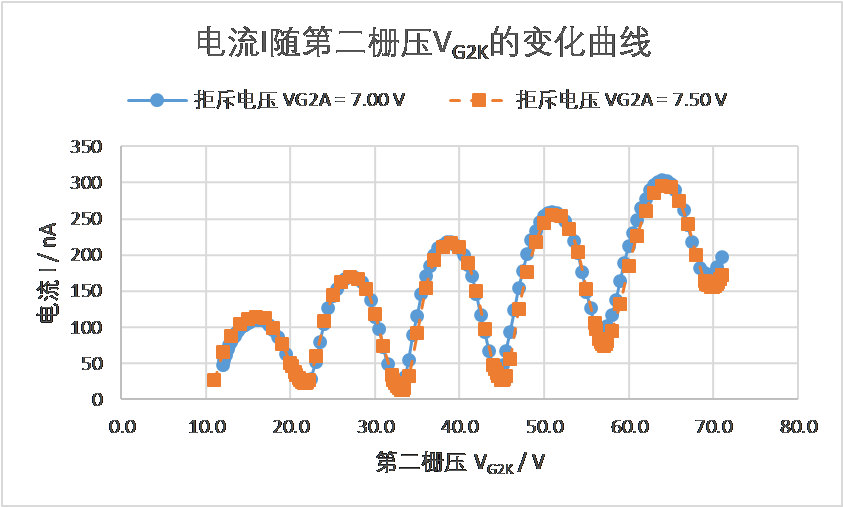
\includegraphics[width=.8\textwidth]{I-VG2K.png}
    \caption{电流$I$随第二栅压$V_{G2K}$的变化曲线.}
    \label{F-1}
\end{figure}

由图\ref{F-1}可见,$I-V_{G2K}$曲线呈现出一种周期性递增、递减交替的变化趋势,但在总体上夫兰克-赫兹管的电流$I$是随着第二栅压$V_{G2K}$. 两条$I-V_{G2K}$曲线的极小值点均呈等间距排列,见表\ref{T-3},且电流极小值随着第二栅压$V_{G2K}$的增大而增大.

\begin{table}[h]
    \centering
    \caption{$I-V_{G2A}$曲线的各个谷值点.}
    \label{T-3}
    \begin{tabular}{|c|c|c|c|c|c|c|c|}
    \hline
    \multicolumn{3}{|c|}{谷值点编号 $i$} & 1 & 2 & 3 & 4 & 5 \\ \hline
    \multirow{2}{*}{拒斥电压 $V_{G2A}$} & 7.00 & \multirow{2}{*}{谷值点电压   $V(i)$ / V} & 21.9 & 33.0 & 44.8 & 56.8 & 68.5 \\ \cline{2-2} \cline{4-8} 
        & 7.50 &  & 21.7 & 33.2 & 45.0 & 57.1 & 69.9 \\ \hline
    % \multicolumn{3}{|c|}{平均谷值点电压 $V(i)$ / V} & 21.8 & 33.1 & 44.9 & 56.9 & 69.2 \\ \hline
    \end{tabular}
\end{table}

比较图\ref{F-1}中两个拒斥电压对应的两条曲线,我们发现部分范围内拒斥电压$V=7.00$ V对应的曲线稍稍高于拒斥电压$V=7.50$ V对应的曲线,且拒斥电压$V=7.50$ V对应的曲线的谷值点稍稍右偏.

电子到达板极形成电流前,除了要与管中气体分子发生碰撞外,还要克服拒斥电压$V_{G2A}$,过大的拒斥电压$V_{G2A}$会导致谷值点偏大,故应该利用拒斥电压$V_{G2A}=7.00$ V下得到的各个谷值点更为准确,由$V(i)=V_{ao}+iV_{el}$,用最小二乘法进行拟合,如图\ref{F-2},得氩原子第一激发电位为$V_{e1}=11.7$ V,查表得氩原子的第一激发电位公认值为$11.5$ V,故本次测量得到的氩原子第一激发电位的相对误差为$(11.7-11.5)/11.5\times 100\%=1.74\%$,符合得较好,从拟合线的截距中还可知夫兰克-赫兹管接触电压(即管内蒸汽与极板之间的接触电势差)为$V_{ao}=9.90$ V.

\begin{figure}[h]
    \centering
    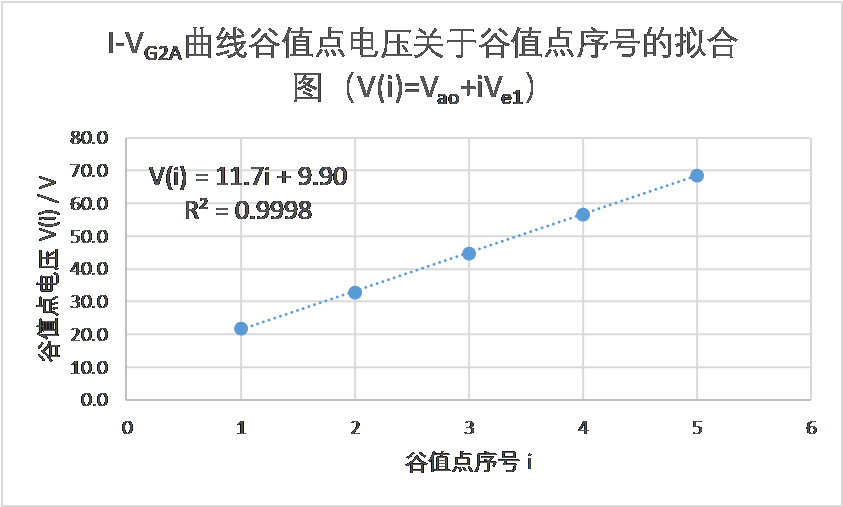
\includegraphics[width=.8\textwidth]{Vi.png}
    \caption{$I-V_{G2A}$曲线谷值点电压关于谷值点序号的拟合图.}
    \label{F-2}
\end{figure}

\section{思考题}
\begin{enumerate}
    \item[1.] 试分析实验中影响$I-V_{G2K}$曲线形状,如峰宽、峰位、峰谷起伏大小及本地电流等的各种因素. 影响第一激发电势测量精度的主要原因是什么?
    (这里所说的“峰宽”、“峰位”实际应该指的是“谷宽”、“谷位”.)
    \begin{enumerate}
        \item \textbf{峰宽}:有两个来源,一个是氩原子能级的\textbf{自然增宽},是一种均匀增宽;另一个是氩原子的麦克斯韦速率分布导致的\textbf{多普勒增宽},是一种非均匀增宽. \textbf{自然增宽}:氩原子第一能级具有一定的寿命$\Delta t$,根据不确定性原理,$\Delta E\cdot\Delta t>\frac{\hbar}{2}$,氩原子第一能级必然有一本征的增宽$\Delta E$,这一增宽效应的线形是洛伦兹分布. \textbf{多普勒增宽}:夫兰克-赫兹管中的氩原子在室温下具有朝各个方向的各个大小的速度,遵循麦克斯韦速度分布率,与电子同方向运动的氩原子需要被速度更大(也就是能量更高)的电子所激发,与电子反方向运动的氩原子则被速度更小(也就是能量更低)的电子激发,多普勒增宽的线形是高斯分布. 实际的峰宽是两种增宽效应的叠加,其线形是Voigt分布曲线(高斯分布和洛伦兹分布的卷积).\\
        影响峰宽的主要因素是夫兰克-赫兹管中的\textbf{气体种类}和\textbf{温度}. 管中气体分子激发态寿命越长,其自然增宽就相应地越窄,$I-V_{G2K}$曲线的峰宽越窄. 并且气体分子质量越大,其麦克斯韦速率分布函数(高斯型函数)的半高宽$2\nu_0\sqrt{\frac{2kT}{mc^2}\ln 2}$就越窄,$I-V_{G2K}$曲线的峰宽越小. 温度越高,一方面导致气体分子间的碰撞频率大大增加,从而处于气体分子的激发态寿命越短,其激发态能级本征的增宽越大,另一方面麦克斯韦速率分布函数的半高宽$2\nu_0\sqrt{\frac{2kT}{mc^2}\ln 2}$越大,这两方面的因素共同作用,会使$I-V_{G2K}$曲线的峰宽变宽.
        \item \textbf{峰位}:由$V(i)=V_{ao}+iV_{e1}$知,$I-V_{G2K}$曲线的峰位主要和管中\textbf{气体种类}和\textbf{两极的金属种类}有关. 其中不同的气体具有不同的激发态能量,也就是对应着不同的$V_{au}$,而不同的电极材料则和管中气体之间有不同的接触电压,也就是对应着不同的$V_{au}$.\\
        此外,由于电子到板极形成电流前,除了要与管中气体分子发生碰撞外,还要克服拒斥电压$V_{G2A}$,过大的\textbf{拒斥电压}$V_{G2A}$会导致谷值点偏大.
        \item \textbf{峰谷起伏大小}:与管中\textbf{气体分子数密度}和\textbf{温度}有关. 管中气体分子数密度越大(即气体越稠密),则电子与气体分子发生碰撞的可能性越大,所以当电子的能量达到气体分子的激发能量时与气体发生非弹性碰撞从而失去动能无法到板极的电子越多,电流下降越明显. 温度越高,如前面所述,多普勒增宽越大,对应的高斯分布函数的高度越小,即处于静止的分子数越少,在电子能量恰好达到气体分子激发能时能与电子发生非弹性碰撞的气体分子越少,电流降低越不明显.
        \item \textbf{本底电流}:本底电流来自于与管中气体分子未发生碰撞或碰撞次数较少从而能到板极的电子. 因此它的影响因素与上一项相同,也是\textbf{气体分子数密度}和\textbf{温度}. 气体分子数越大,温度越低,则本底电流越小.
        此外,\textbf{第二栅压}$V_{G2K}$越大,本底电流越大,这是因为第二栅压$V_{G2K}$越大,电子的动能越大,所以在与气体分子碰撞几率一定的情况下,更可能留有足够的能量达到板极而形成电流.
    \end{enumerate}
    影响第一激发电势测量精度的主要因素:\textbf{拒斥电压}$V_{G2A}$和\textbf{温度}. 拒斥电压越小,则峰位偏离越小,信号越强,温度越低,则多普勒展宽越小,精度越高.
    \item[2.] 试分析电子同原子碰撞时的能量转移和电子动能关系,解释夫兰克-赫兹实验观察原子第一激发态的物理过程.\\
    当电子的能量小于原子第一激发态与其基态的能量差$E_2-E_1$时,即使电子在运动过程中与原子相碰撞也只有微小的能量交换(弹性碰撞,因为电子质量远远小于原子质量,故动能改变很小);而当电子的能量等于或稍大于原子的第一激发态与其基态的能量差$E_2-E_1$时,若电子与原子相碰撞,则电子很有可能将等于$E_2-E_1$的动能传给原子,而将原子从基态激发到第一激发态.\\
    夫兰克-赫兹实验中,电子从热阴极发出,被阴极$K$和第二栅极$G_2$之间的加速电压$V_{G2K}$加速,在板极和第二栅极$G_2$之间加有反向拒斥电压$V_{G2A}$. 当电子通过$KG_2$空间进入$G_2A$空间时,如果有足够大的能量($\leq eV_{G2A}$),就能克服反向拒斥电压而到板极形成电流;若电子在$KG_2$空间与原子碰撞,将一部分能量转移到原子上,则可能由于所剩动能不足以克服拒斥电压而无法达到板极形成电流.逐渐增大第二栅压$V_{G2K}$,电子在$V_{G2K}$间被加速达到的动能也逐渐增大,电流逐渐增大;当电子的动能第一次被加速到$E_2-E_1$时,电子与原子发生非弹性碰撞损失动能,从而无法达到极板形成电流,导致电流下降;继续增大第二栅压$V_{G2K}$,电子的动能继续增大,从而在第一次与原子发生碰撞后有更大的剩余动能,因此电流开始重新上升;直至其动能达到两倍的电流$E_2-E_1$,导致电子可以与原子发生两次非弹性碰撞,电流再次下降. 如此循环往复,可以得到随第二栅压$V_{G2K}$周期性交替增加和减弱的电流,电流的两个谷值点间的电压对应的能量即为原子的第一激发态与其基态之间的能量差.
\end{enumerate}

\section*{附录}
\begin{table}[h]
    \centering
    \caption{拒斥电压$V_{G2A}=7.00$ V时,电流I随第二栅压$V_{G2K}$的变化情况}
    \label{T-1}
    \begin{tabular}{|c|c|c|c|c|c|c|c|c|c|}
    \hline
    \begin{tabular}[c]{@{}c@{}}第二栅压\\ $V_{G2K}$ / V\end{tabular} & \begin{tabular}[c]{@{}c@{}}电流\\ $I$ / nA\end{tabular} & \begin{tabular}[c]{@{}c@{}}第二栅压\\ $V_{G2K}$ / V\end{tabular} & \begin{tabular}[c]{@{}c@{}}电流\\ $I$ / nA\end{tabular} & \begin{tabular}[c]{@{}c@{}}第二栅压\\ $V_{G2K}$ / V\end{tabular} & \begin{tabular}[c]{@{}c@{}}电流\\ $I$ / nA\end{tabular} & \begin{tabular}[c]{@{}c@{}}第二栅压\\ $V_{G2K}$ / V\end{tabular} & \begin{tabular}[c]{@{}c@{}}电流\\ $I$ / nA\end{tabular} & \begin{tabular}[c]{@{}c@{}}第二栅压\\ $V_{G2K}$ / V\end{tabular} & \begin{tabular}[c]{@{}c@{}}电流\\ $I$ / nA\end{tabular} \\ \hline
    12.0 & 48 & 18.0 & 96 & 30.5 & 97 & 43.5 & 67 & 57.5 & 101 \\ \hline
    12.2 & 55 & 18.5 & 86 & 31.0 & 72 & 44.0 & 46 & 58.0 & 117 \\ \hline
    12.4 & 61 & 19.0 & 76 & 31.5 & 49 & 44.5 & 35 & 58.5 & 137 \\ \hline
    12.6 & 70 & 19.5 & 63 & 32.0 & 34 & 45.0 & 35 & 59.0 & 164 \\ \hline
    12.8 & 75 & 20.0 & 50 & 32.5 & 21 & 45.2 & 47 & 59.5 & 189 \\ \hline
    13.0 & 79 & 20.5 & 38 & 32.7 & 19 & 45.5 & 67 & 60.0 & 212 \\ \hline
    13.2 & 85 & 21.0 & 30 & 32.9 & 17 & 46.0 & 93 & 60.5 & 230 \\ \hline
    13.4 & 88 & 21.2 & 28 & 33.0 & 16 & 46.5 & 123 & 61.0 & 248 \\ \hline
    13.6 & 91 & 21.4 & 25 & 33.2 & 17 & 47.0 & 154 & 61.5 & 265 \\ \hline
    13.8 & 94 & 21.6 & 24 & 33.4 & 24 & 47.5 & 177 & 62.0 & 277 \\ \hline
    14.0 & 98 & 21.8 & 23 & 33.6 & 31 & 48.0 & 201 & 62.5 & 289 \\ \hline
    14.2 & 100 & 21.9 & 23 & 34.0 & 55 & 48.5 & 220 & 63.0 & 297 \\ \hline
    14.4 & 101 & 22.0 & 23 & 34.5 & 89 & 49.0 & 233 & 63.5 & 301 \\ \hline
    14.6 & 103 & 22.2 & 24 & 35.0 & 115 & 49.5 & 245 & 64.0 & 303 \\ \hline
    14.8 & 105 & 22.4 & 28 & 35.5 & 145 & 50.0 & 253 & 64.5 & 302 \\ \hline
    15.0 & 106 & 23.0 & 51 & 36.0 & 170 & 50.5 & 258 & 65.0 & 298 \\ \hline
    15.2 & 107 & 23.5 & 79 & 36.5 & 185 & 51.0 & 259 & 65.5 & 289 \\ \hline
    15.4 & 108 & 24.0 & 104 & 37.0 & 200 & 51.5 & 258 & 66.0 & 276 \\ \hline
    15.6 & 109 & 24.5 & 126 & 37.5 & 209 & 52.0 & 254 & 66.5 & 262 \\ \hline
    15.8 & 110 & 25.0 & 143 & 38.0 & 214 & 52.5 & 246 & 67.0 & 241 \\ \hline
    16.0 & 110 & 25.5 & 153 & 38.5 & 217 & 53.0 & 236 & 67.5 & 218 \\ \hline
    16.1 & 110 & 26.0 & 161 & 39.0 & 217 & 53.5 & 219 & 68.0 & 200 \\ \hline
    16.2 & 110 & 26.5 & 167 & 39.5 & 214 & 54.0 & 202 & 68.5 & 182 \\ \hline
    16.3 & 110 & 27.0 & 169 & 40.0 & 209 & 54.5 & 176 & 69.0 & 174 \\ \hline
    16.4 & 110 & 27.5 & 169 & 40.5 & 200 & 55.0 & 149 & 69.2 & 173 \\ \hline
    16.5 & 110 & 28.0 & 167 & 41.0 & 186 & 55.5 & 126 & 69.4 & 172 \\ \hline
    16.6 & 110 & 28.5 & 162 & 41.5 & 170 & 56.0 & 102 & 69.6 & 171 \\ \hline
    16.7 & 109 & 29.0 & 153 & 42.0 & 146 & 56.5 & 87 & 69.8 & 172 \\ \hline
    17.0 & 108 & 29.5 & 138 & 42.5 & 117 & 57.0 & 87 & 70.0 & 173 \\ \hline
    17.5 & 103 & 30.0 & 114 & 43.0 & 93 & 57.2 & 93 & 70.5 & 183 \\ \hline
        &  &  &  &  &  &  &  & 71.0 & 197 \\ \hline
    \end{tabular}
\end{table}

\begin{table}[h]
    \centering
    \caption{拒斥电压$V_{G2A}=7.50$ V时,电流I随第二栅压$V_{G2K}$的变化情况}
    \label{T-2}
    \begin{tabular}{|c|c|c|c|c|c|c|c|}
    \hline
    \begin{tabular}[c]{@{}c@{}}第二栅压\\ $V_{G2K}$ / V\end{tabular} & \begin{tabular}[c]{@{}c@{}}电流\\ $I$ / nA\end{tabular} & \begin{tabular}[c]{@{}c@{}}第二栅压\\ $V_{G2K}$ / V\end{tabular} & \begin{tabular}[c]{@{}c@{}}电流\\ $I$ / nA\end{tabular} & \begin{tabular}[c]{@{}c@{}}第二栅压\\ $V_{G2K}$ / V\end{tabular} & \begin{tabular}[c]{@{}c@{}}电流\\ $I$ / nA\end{tabular} & \begin{tabular}[c]{@{}c@{}}第二栅压\\ $V_{G2K}$ / V\end{tabular} & \begin{tabular}[c]{@{}c@{}}电流\\ $I$ / nA\end{tabular} \\ \hline
    11.0 & 26 & 27 & 169 & 44.2 & 42 & 57.5 & 80 \\ \hline
    12.0 & 65 & 28 & 167 & 44.4 & 36 & 58.0 & 95 \\ \hline
    13.0 & 88 & 29 & 153 & 44.6 & 32 & 59.0 & 132 \\ \hline
    14.0 & 104 & 30 & 118 & 44.9 & 26 & 60.0 & 184 \\ \hline
    15.0 & 111 & 31 & 73 & 45.1 & 26 & 61.0 & 226 \\ \hline
    16.0 & 114 & 32 & 34 & 45.3 & 28 & 62.0 & 260 \\ \hline
    17.0 & 112 & 32 & 26 & 45.5 & 32 & 63.0 & 285 \\ \hline
    18.0 & 99 & 32 & 22 & 46.0 & 56 & 64.0 & 295 \\ \hline
    19.0 & 77 & 33 & 19 & 47.0 & 125 & 65.0 & 293 \\ \hline
    20.0 & 50 & 33 & 15 & 48.0 & 176 & 66.0 & 274 \\ \hline
    20.2 & 46 & 33 & 13 & 49.0 & 217 & 67.0 & 242 \\ \hline
    20.5 & 38 & 33 & 13 & 50.0 & 244 & 68.0 & 200 \\ \hline
    20.7 & 34 & 34 & 15 & 51.0 & 255 & 69.0 & 163 \\ \hline
    21.0 & 30 & 34 & 32 & 52.0 & 253 & 69.2 & 160 \\ \hline
    21.2 & 27 & 35 & 92 & 53.0 & 236 & 69.4 & 158 \\ \hline
    21.4 & 24 & 36 & 154 & 54.0 & 204 & 69.7 & 156 \\ \hline
    21.6 & 23 & 37 & 192 & 55.0 & 153 & 69.9 & 156 \\ \hline
    21.8 & 23 & 38 & 211 & 56.0 & 105 & 70.0 & 156 \\ \hline
    22.0 & 24 & 39 & 216 & 56.2 & 97 & 70.2 & 157 \\ \hline
    22.2 & 27 & 40 & 210 & 56.5 & 84 & 70.4 & 159 \\ \hline
    23.0 & 60 & 41 & 188 & 56.7 & 79 & 70.6 & 162 \\ \hline
    24.0 & 108 & 42 & 150 & 56.9 & 76 & 70.8 & 166 \\ \hline
    25.0 & 144 & 43 & 97 & 57.1 & 74 & 71.0 & 172 \\ \hline
    26.0 & 162 & 44 & 48 & 57.3 & 76 &  &  \\ \hline
    \end{tabular}
\end{table}
\end{document}